This first approach is most similar to Sequential Deep Belief Networks in that it learns a transition operator between hidden latent states \(H\). This model uses the power of GSN's to learn hidden representations that vastly reduce the complexity of the input data space, making transitions between data manifolds at higher layers of representation much easier to model. Therefore, the transition step of learning \(H \rightarrow H\) over time should be less complicated (i.e. only needing a single linear regression step between hidden states). This model trains by alternating over two versions of the dataset:
\begin{enumerate}
\item A generative Gibbs sampling pass for \(k\) samples on each input in arbitrary order (for the GSN to learn the data manifolds)
\item A real time-sequenced order of the input to learn the regression \(H \rightarrow H\)
\end{enumerate}
Alternating between training the GSN parameters on the generative input sequence through Gibbs sampling and learning the hidden state transition operator on the real sequence of inputs allows the model to tune parameters quickly in an expectation-maximization style of training.



\section{Recurrent nature of deep GSNs}

While GSNs are inherently recurrent and depend on the previous latent and visible states to determine the current hidden state, \(H_{t} \sim P_{\Theta_1}(H|H_{t-1},X_{t-1})\), this ordering \(t\) is generated through the GSN Gibbs sampling process and does not reflect the real sequence of inputs over time. Using this sampling process, GSNs actively mix between modes that are close together in the input space, not the sequential space. For example, a GSN trained on MNIST data will learn to mix well between the modes of digits that look similar in the pixel space - sampling from the digit ``4" transitions to a ``9", etc.

\begin{figure}[h!]
  \centering
    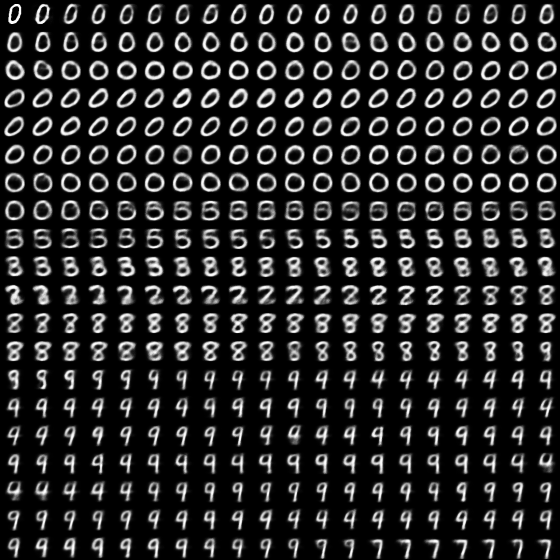
\includegraphics[width=0.8\textwidth]{gsn_samples}
\caption{Samples from GSN after 290 training epochs. Good mixing between major modes in the input space.}
\end{figure}

To learn transitions between sequential modes in the input space, both  the \(t\) from the GSN sampling process and the sequential \(t_{real}\) from the input data sequence need to be utilized.


\section{Algorithm}

This model's training algorithm is similar to expectation maximization (EM) - first optimizing GSN parameters over the input data, then learning the transition \(H \rightarrow H\) parameters, and repeating. After the initial GSN pass over the data, training the GSN parameters becomes more powerful as the reconstruction cost of the current input as well as the next predicted input are both used for computing the gradients.

\begin{algorithm}[h!]
	\KwIn{training set \(D\) of examples \(X\) in sequential order, \(N\) layers, \(k\) walkbacks}
	Initialize GSN parameters \(\Theta_{GSN} = \) \{List(weights from one layer to the next), List(bias for layer))\}\;
	Initialize transition parameters \(\Theta_{transition}=\) \{List(identity matrix for layer), List(bias for layer)\} \;
	\While{training not converged}{
		\For{each input \(X\)}{
			Sample GSN for \(k\) walkbacks, creating \(k^*(X,X_{recon})\) training pairs\;
			Transition from ending hidden states \(H\) to next predicted hidden states \(H'\) with transition parameters \(\Theta_{transition}\)\;
			Sample GSN again for \(k\) walkbacks, creating  \(k^*(X',X'_{recon})\) training pairs\;
			Train GSN parameters \(\Theta_{GSN}\) using these pairs, keeping \(\Theta_{transition}\) fixed\;
		}
		\For{each input \(X\)}{
			Sample GSN for \(k\) walkbacks, creating ending hidden states \(H\)\;
			Transition from ending hidden states \(H\) to next predicted hidden states \(H'\) with transition parameters \(\Theta_{transition}\)\;
			Sample GSN again for \(k\) walkbacks, creating the ending \((X',X'_{recon})\) pair\;
			Train transition parameters \(\Theta_{transition}\) with this pair, keeping \(\Theta_{GSN}\) fixed\;
		}
	}
	\caption{ Model 1 EM Algorithm }
\end{algorithm}

\section{Experimental results}

This algorithm was tested on artificially sequenced MNIST handwritten digit data. The dataset was sequenced by ordering the inputs 0-9 repeating. The GSN uses hyperbolic tangent (tanh) activation with 3 hidden layers of 1500 nodes and sigmoidal activation for the visible layer. For the GSN, Gaussian noise is added pre- and post-activation with a mean of 0 and a sigma of 2, and input corruption noise is salt-and-pepper. Training was performed for 300 iterations over the input data using a batch size of 100, with a learning rate of 0.25, annealing rate of 0.995, and momentum of 0.5.

This model achieved a binary cross-entropy of 0.1651 for reconstructing the current input  and 0.2317 for reconstructing the predicted next input after 300 epochs. An interesting result is that the predicted reconstruction of the next digits appears to be close to the average of that digit, which makes sense given the training set was shuffled and re-ordered after every epoch.

\begin{figure}[h!]
  \centering
    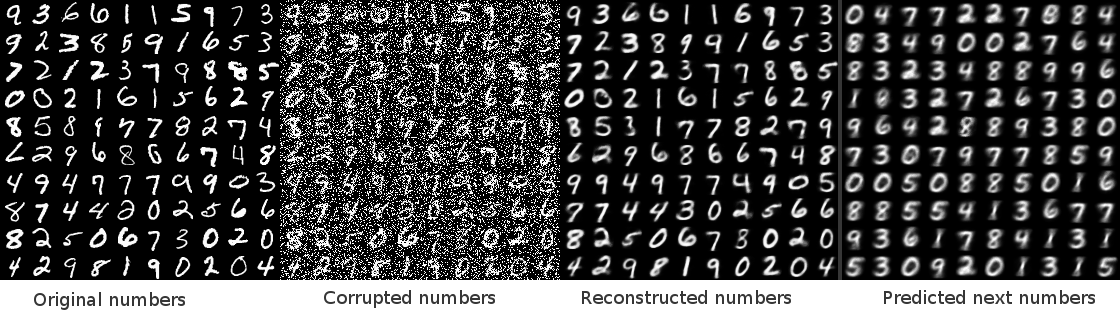
\includegraphics[width=1.0\textwidth]{story1_reconstruction}
\caption{Model 1 reconstruction of digits and predicted next digits after 300 iterations.}
\end{figure}

\begin{figure}[h!]
  \centering
    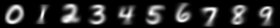
\includegraphics[width=0.5\textwidth]{average_mnist_train}
\caption{Average MNIST training data by digit.}
\end{figure}

Differences between the predicted next number and the average number seem to occur when the GSN incorrectly reconstructs the original corrupted input. These results provide evidence that the original assumption is correct: the GSN learns representations that disentangle complex input data, which allows a simple regression step to predict the next input in a linear manner. A comparison of results is included in the Discussion.

Sampling in the input space is similar to a GSN:
\begin{figure}[h!]
  \centering
    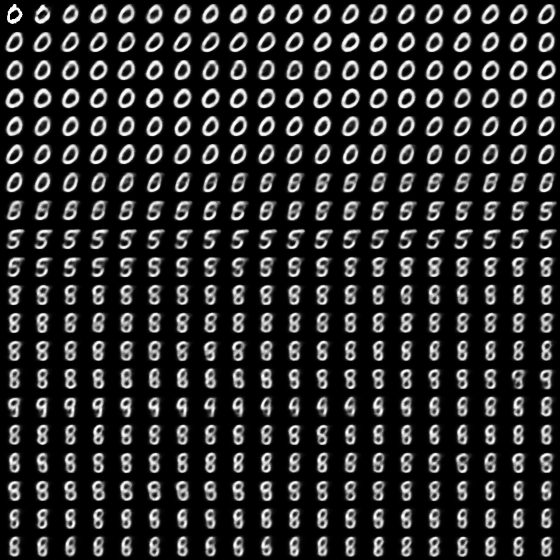
\includegraphics[width=.8\textwidth]{story1_samples_100}
\caption{Model 1 sampling after 90 training iterations; smooth mixing between major modes.}
\end{figure}
